\chapter{Discussion and Conclusion}

\section{Interpretation of Results}
The implementation and preliminary results of Medibot demonstrate substantial advancements in AI-driven medical diagnostics. The system's robust architecture, encompassing both computer vision and large language models, has shown promising results in terms of accuracy and efficiency. Medibot’s ability to process and interpret complex medical data through its sophisticated algorithms underlines the potential of AI to support and enhance decision-making in healthcare settings.

\subsection{Challenges and Limitations}
The development of Medibot has encountered several significant challenges, key among them being the scarcity and unstructured nature of available medical data. To overcome this, we were compelled to generate our own datasets using large language models, which introduced additional complexities related to data validity and representativeness.

\begin{itemize}
    \item \textbf{Data Acquisition and Structure:} Obtaining sufficient medical data for training our models proved challenging due to the proprietary nature of most medical datasets. Moreover, much of the available data lacked the structured format necessary for efficient processing and analysis, necessitating extensive preprocessing and data structuring efforts using advanced language models.
    \item \textbf{Bias and Model Reliability:} To mitigate bias in our models, we employed multiple algorithms and diverse data sources. Despite these efforts, ensuring the complete neutrality and fairness of the models remains a complex challenge that requires ongoing attention and refinement.
    \item \textbf{Computational Resources:} Limited access to computational resources and funding constraints significantly impacted our ability to experiment with various architectures and training methodologies. This limitation affected our capacity to iterate quickly and test the most innovative AI techniques.
    \item \textbf{System Integration:} The multimodal nature of Medibot introduced complexities in integrating various components such as text processing units, image analysis models, and user interface elements. Ensuring seamless interaction between these diverse systems was both challenging and resource-intensive.
\end{itemize}

These challenges underscore the difficulties in deploying advanced AI systems in healthcare settings, which require not only technological innovation but also a deep understanding of the regulatory and ethical dimensions of medical practice.

\section{Support from Microsoft Azure Founders Fund}
On June 18, 2024, Medibot was awarded a significant endorsement from the Microsoft Azure Founders Fund, receiving \$5000 in Azure credits. This grant, valid for one year, underscores Microsoft's confidence in Medibot's potential to revolutionize medical diagnostics with AI-driven solutions. The Azure credits will empower us to harness Microsoft Azure's robust cloud computing services, enabling enhanced processing capabilities and scalability. This support is pivotal in advancing our development, allowing us to integrate more sophisticated AI features and expand our service offerings, thereby accelerating our mission to deliver advanced healthcare solutions.

\begin{figure}[H]
    \centering
    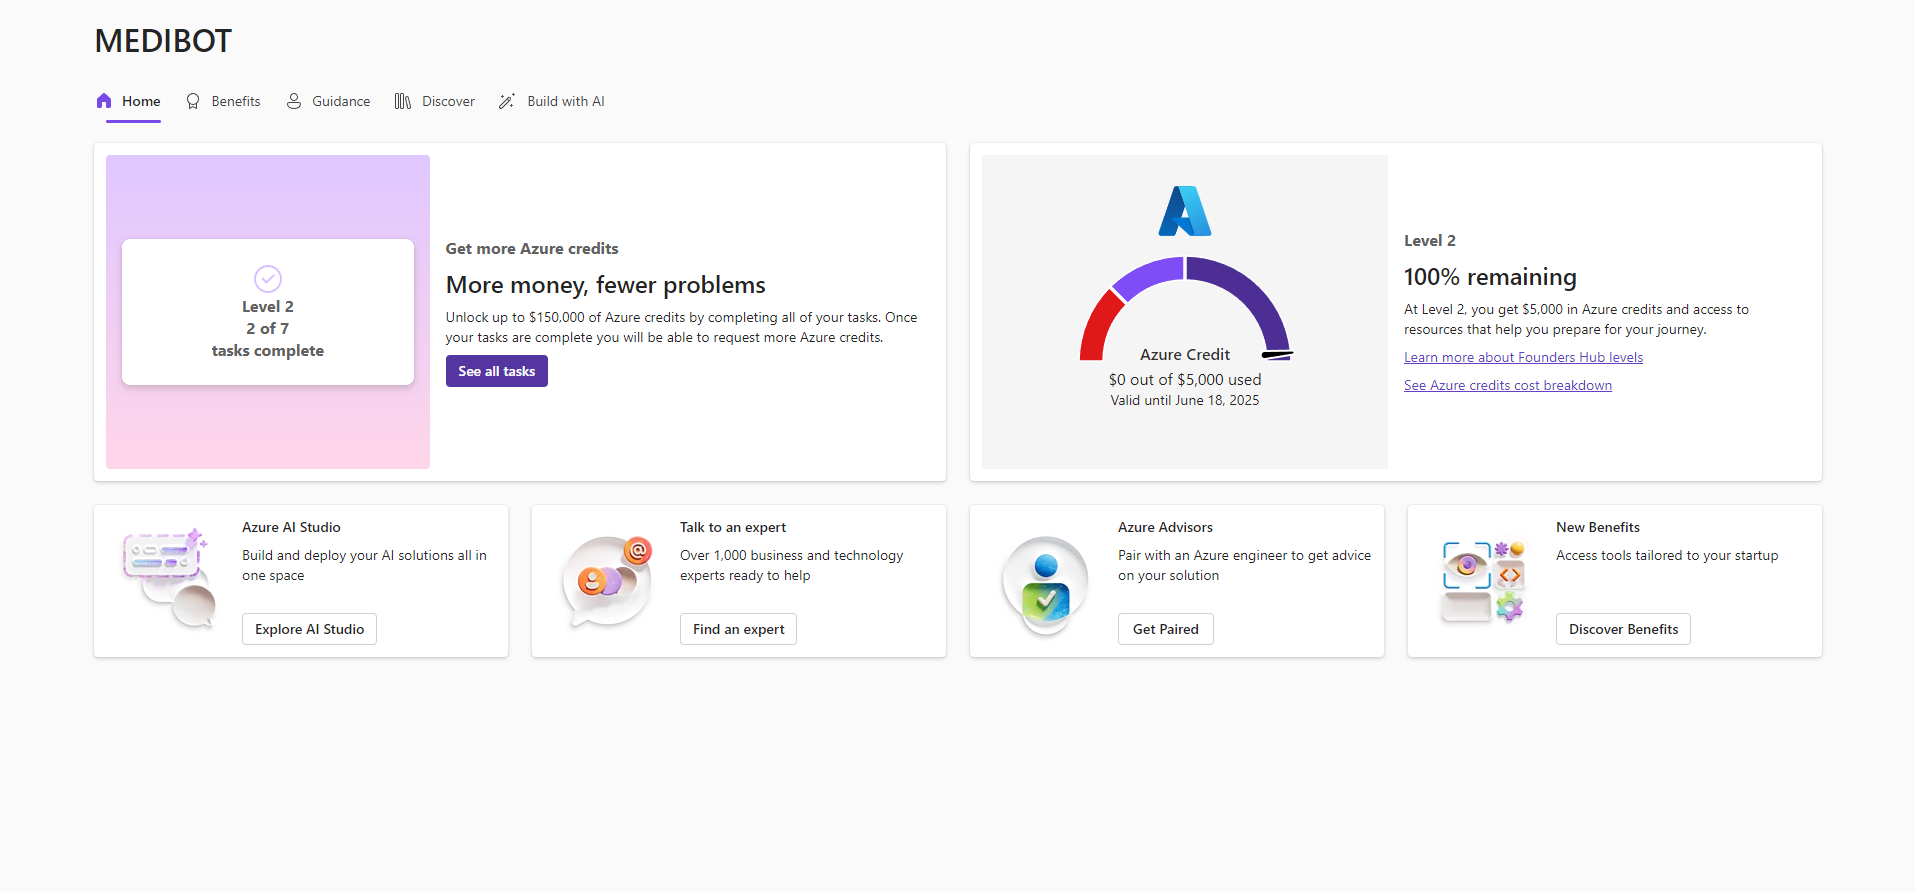
\includegraphics[width=\textwidth]{./Figures/azurefund.png}
    \caption{Microsoft Azure Founders Fund Approval Dashboard}
    \label{fig:azure_fund}
\end{figure}

\section{Future Work}
In light of our current achievements, the challenges faced, and the recent financial support from Microsoft Azure Founders Fund, our future efforts will encompass:

\begin{itemize}
    \item \textbf{Enhancing Model Accuracy:} With the additional Azure credits, we plan to access more substantial computational resources, enabling us to continuously train our models with up-to-date and diverse datasets. This effort will improve diagnostic accuracy, reduce biases, and allow us to explore more complex model architectures.
    \item \textbf{Expanding System Capabilities:} We aim to integrate additional functionalities such as real-time patient monitoring, predictive analytics for chronic diseases, and a new voice-to-text feature to enhance user interaction by allowing spoken input, facilitating accessibility and ease of use.
    \item \textbf{Interoperability:} Ensuring Medibot can seamlessly integrate with existing healthcare IT ecosystems is crucial. With enhanced resources, we can accelerate the development of interoperable solutions, facilitating widespread adoption.
    \item \textbf{Global Expansion:} The fund also opens up possibilities for localizing Medibot to cater to non-English speaking regions and adapting the system to meet various international healthcare standards. This will help in addressing the nuances of global healthcare challenges.
    \item \textbf{Big Data Capabilities:} The Azure funding will enable us to handle larger datasets, which are essential for training more robust models. This capability will directly address our previous challenges of limited data access and allow for more extensive testing and validation phases.
    \item \textbf{Enhanced Image Processing:} We plan to augment our image processing capabilities by incorporating additional data points such as age, gender, and position of view from image metadata. This enhancement will improve the specificity and relevance of our diagnostic models.
    \item \textbf{Training Larger MoE Models:} With the capability to handle more computational resources, we aim to train larger MoE (Mixture of Experts) 22b*8 models. Their high contextual awareness can yield better results across various medical query types and scenarios.
\end{itemize}

These initiatives will leverage the new funding to significantly scale Medibot’s capabilities, pushing the boundaries of what our AI-driven solution can achieve in the medical field.


\section{Conclusion}

Medibot, our Medical Diagnosis AI Assistant, represents a transformative approach in healthcare, merging advanced AI technologies with medical diagnostics to provide immediate, accessible, and accurate medical advice. Throughout its development, we have integrated state-of-the-art machine learning models, sophisticated natural language processing tools, and innovative computer vision capabilities to create a system that not only understands complex medical language but also interprets medical imagery with high precision.

The implementation of Medibot involved several components, each carefully crafted to address specific needs within the healthcare sector. The frontend, developed using ReactJS and TypeScript, offers a user-friendly interface that simplifies the interaction process for users. The backend, powered by Node.js and MongoDB, ensures efficient data handling and robust API management, allowing Medibot to handle multiple user interactions seamlessly. The integration of Large Language Models (LLMs) and Computer Vision systems has equipped Medibot with the ability to process textual and visual data effectively, turning raw medical data into actionable insights.

One of the critical achievements of this project has been the adaptation and fine-tuning of models like Llama3-8b and Llama3-70b, which have significantly enhanced Medibot's ability to provide tailored medical advice and handle diverse medical inquiries. Moreover, the support from Microsoft Azure Founders Fund has been instrumental, providing us with the necessary resources to scale our operations, train more complex models, and expand our dataset capacities.

Despite these advancements, we encountered challenges such as limited initial data access, the need to generate synthetic medical data, and the complexities of integrating multimodal systems. However, the Azure grant has positioned us to overcome these hurdles by allowing access to enhanced computational resources and enabling global scaling and multilingual capabilities.

Future work for Medibot includes expanding its real-time patient monitoring features, developing voice-to-text capabilities, enhancing interoperability with existing medical systems, and extending our services to non-English speaking regions. Additionally, plans to integrate predictive analytics for chronic diseases and improve model accuracies with more extensive and diverse datasets will further refine Medibot’s functionalities.

In conclusion, Medibot stands as a testament to the potential of artificial intelligence in revolutionizing healthcare. It exemplifies how technology can bridge gaps in medical service delivery, providing reliable, efficient, and accessible diagnostics and patient care. As we continue to develop and expand Medibot, we aim to not only enhance its capabilities but also ensure it becomes an integral part of the global healthcare ecosystem, making high-quality medical advice available to everyone, everywhere.
